\documentclass[12pt]{report}\usepackage[]{graphicx}\usepackage[dvipsnames]{xcolor}
% maxwidth is the original width if it is less than linewidth
% otherwise use linewidth (to make sure the graphics do not exceed the margin)
\makeatletter
\def\maxwidth{ %
  \ifdim\Gin@nat@width>\linewidth
    \linewidth
  \else
    \Gin@nat@width
  \fi
}
\makeatother

\definecolor{fgcolor}{rgb}{0.345, 0.345, 0.345}
\newcommand{\hlnum}[1]{\textcolor[rgb]{0.686,0.059,0.569}{#1}}%
\newcommand{\hlstr}[1]{\textcolor[rgb]{0.192,0.494,0.8}{#1}}%
\newcommand{\hlcom}[1]{\textcolor[rgb]{0.678,0.584,0.686}{\textit{#1}}}%
\newcommand{\hlopt}[1]{\textcolor[rgb]{0,0,0}{#1}}%
\newcommand{\hlstd}[1]{\textcolor[rgb]{0.345,0.345,0.345}{#1}}%
\newcommand{\hlkwa}[1]{\textcolor[rgb]{0.161,0.373,0.58}{\textbf{#1}}}%
\newcommand{\hlkwb}[1]{\textcolor[rgb]{0.69,0.353,0.396}{#1}}%
\newcommand{\hlkwc}[1]{\textcolor[rgb]{0.333,0.667,0.333}{#1}}%
\newcommand{\hlkwd}[1]{\textcolor[rgb]{0.737,0.353,0.396}{\textbf{#1}}}%
\let\hlipl\hlkwb

\usepackage{framed}
\makeatletter
\newenvironment{kframe}{%
 \def\at@end@of@kframe{}%
 \ifinner\ifhmode%
  \def\at@end@of@kframe{\end{minipage}}%
  \begin{minipage}{\columnwidth}%
 \fi\fi%
 \def\FrameCommand##1{\hskip\@totalleftmargin \hskip-\fboxsep
 \colorbox{shadecolor}{##1}\hskip-\fboxsep
     % There is no \\@totalrightmargin, so:
     \hskip-\linewidth \hskip-\@totalleftmargin \hskip\columnwidth}%
 \MakeFramed {\advance\hsize-\width
   \@totalleftmargin\z@ \linewidth\hsize
   \@setminipage}}%
 {\par\unskip\endMakeFramed%
 \at@end@of@kframe}
\makeatother

\definecolor{shadecolor}{rgb}{.97, .97, .97}
\definecolor{messagecolor}{rgb}{0, 0, 0}
\definecolor{warningcolor}{rgb}{1, 0, 1}
\definecolor{errorcolor}{rgb}{1, 0, 0}
\newenvironment{knitrout}{}{} % an empty environment to be redefined in TeX

\usepackage{alltt}

\usepackage[utf8]{inputenc}
\usepackage[spanish]{babel}
\usepackage[margin=2.54cm]{geometry}
\usepackage[dvipsnames]{xcolor}
\usepackage{array, amssymb, amsthm, enumitem, fancyhdr, float, graphicx, hyperref, hologo, mathtools, tikz, tikz-cd}
\usepackage[spanish, noabbrev]{cleveref}

\pagestyle{fancy}
\lhead{\footnotesize \leftmark}
\rhead{\footnotesize \rightmark}

\title{
	\huge
	\noindent\textbf{Fundamentos de la Ciencia de Datos}\\
	
	{\Large \textit{Práctica 1}}
	\vspace{1cm}
	
	\huge
	Grado en Ingeniería Informática\\
	Universidad de Alcalá\\
	
	\vspace{1cm}
	
	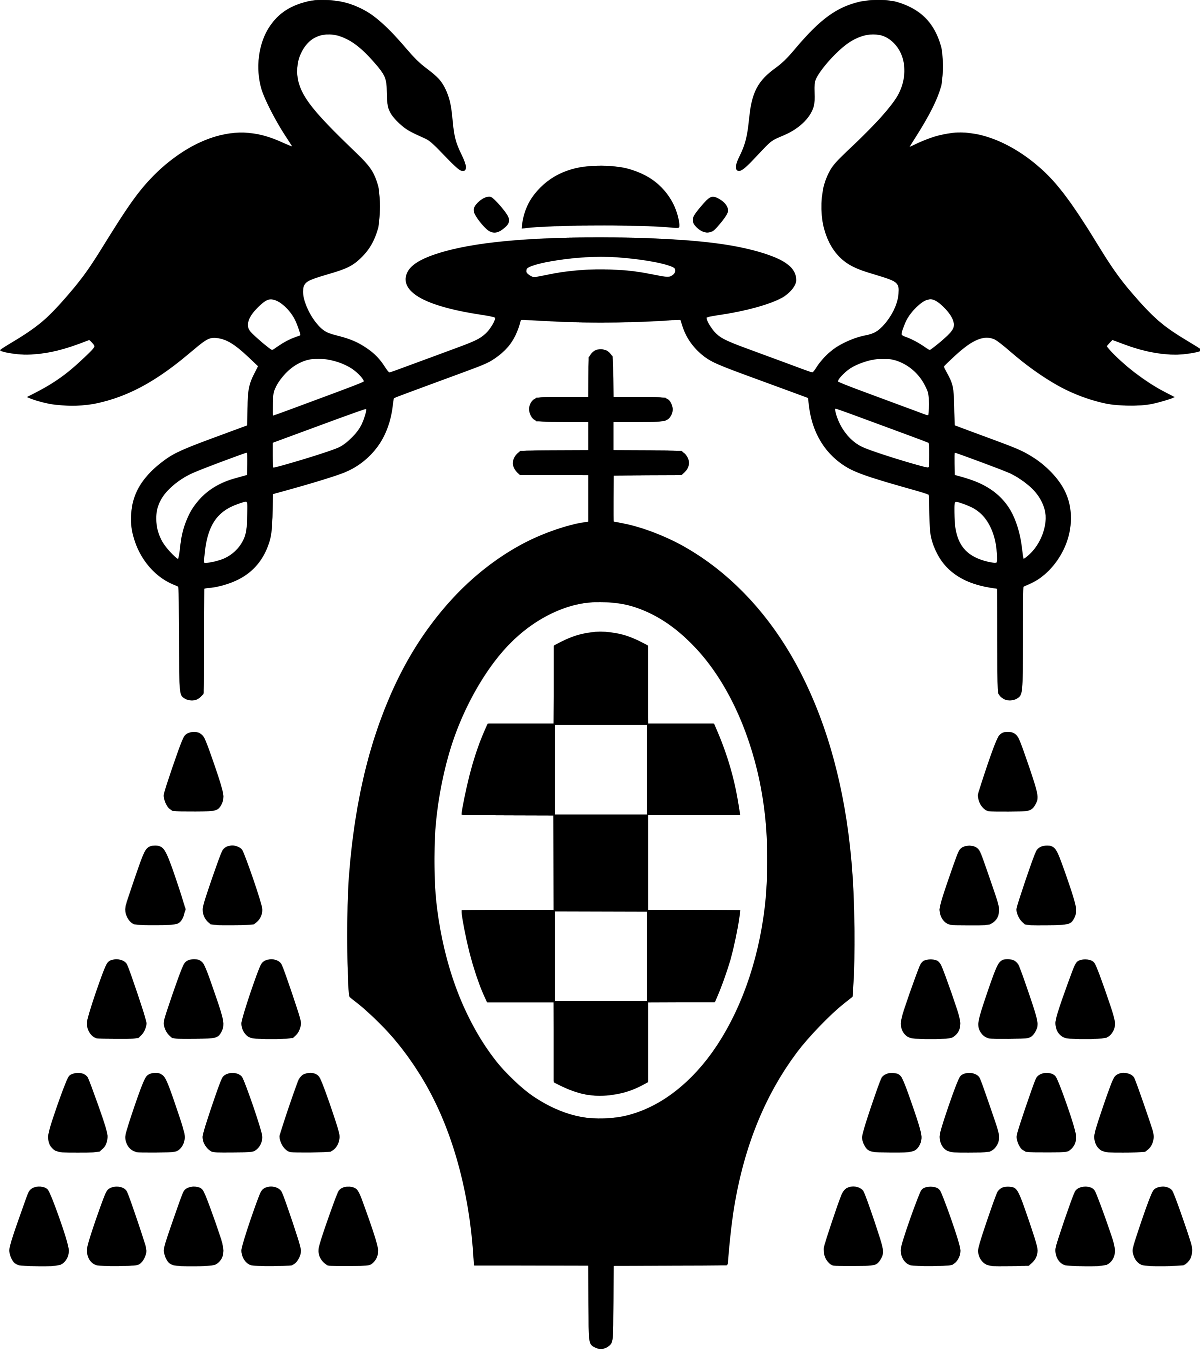
\includegraphics[scale=0.075]{img/logo}
}

\author{
	Pablo García García\\
	Abel López Martínez\\
	Álvaro Jesús Martínez Parra\\
	Raúl Moratilla Núñez
}

\date{
	\large{14 de noviembre de 2023}
}

\hypersetup{
	pdftitle={Práctica 1}, 
	pdfauthor={Pablo García García, Abel López Martínez, Álvaro Jesús Martínez Parra, Raúl Moratilla Núñez}, 
	pdfsubject={Fundamentos de la Ciencia de Datos}, 
	pdfcenterwindow, 
	pdfnewwindow=true, 
	pdfkeywords={Entrega de la PL1 de laboratorio correspondiente al Curso 2023-2024}, 
	bookmarksopen=true 
}
\IfFileExists{upquote.sty}{\usepackage{upquote}}{}
\begin{document}
	
\begin{knitrout}
\definecolor{shadecolor}{rgb}{0.969, 0.969, 0.969}\color{fgcolor}\begin{kframe}
\begin{alltt}
\hlstd{fichero} \hlkwb{=} \hlkwd{read.csv}\hlstd{(}\hlstr{"distancia_universitarios.csv"}\hlstd{)}
\hlstd{fichero}
\end{alltt}
\begin{verbatim}
##    Distancia
## 1       16.5
## 2       34.8
## 3       20.7
## 4        6.2
## 5        4.4
## 6        3.4
## 7       24.0
## 8       24.0
## 9       32.0
## 10      30.0
## 11      33.0
## 12      27.0
## 13      15.0
## 14       9.4
## 15       2.1
## 16      34.0
## 17      24.0
## 18      12.0
## 19       4.4
## 20      28.0
## 21      31.4
## 22      21.6
## 23       3.1
## 24       4.5
## 25       5.1
## 26       4.0
## 27       3.2
## 28      25.0
## 29       4.5
## 30      20.0
## 31      34.0
## 32      12.0
## 33      12.0
## 34      12.0
## 35      12.0
## 36       5.0
## 37      19.0
## 38      30.0
## 39       5.5
## 40      38.0
## 41      25.0
## 42       3.7
## 43       9.0
## 44      30.0
## 45      13.0
## 46      30.0
## 47      30.0
## 48      26.0
## 49      30.0
## 50      30.0
## 51       1.0
## 52      26.0
## 53      22.0
## 54      10.0
## 55       9.7
## 56      11.0
## 57      24.1
## 58      33.0
## 59      17.2
## 60      27.0
## 61      24.0
## 62      27.0
## 63      21.0
## 64      28.0
## 65      30.0
## 66       4.0
## 67      46.0
## 68      29.0
## 69       3.7
## 70       2.7
## 71       8.1
## 72      19.0
## 73      16.0
\end{verbatim}
\begin{alltt}
\hlstd{len} \hlkwb{=} \hlkwa{function}\hlstd{(}\hlkwc{list}\hlstd{)\{}
        \hlstd{count} \hlkwb{=} \hlnum{0}
        \hlkwa{for} \hlstd{(element} \hlkwa{in} \hlstd{list)\{}
                \hlstd{count} \hlkwb{=} \hlstd{count} \hlopt{+} \hlnum{1}
        \hlstd{\}}
        \hlstd{count}
\hlstd{\}}

\hlstd{distancias} \hlkwb{=} \hlstd{fichero}\hlopt{$}\hlstd{Distancia}

\hlstd{longitud} \hlkwb{=} \hlkwd{len}\hlstd{(distancias)}
\hlstd{longitud}
\end{alltt}
\begin{verbatim}
## [1] 73
\end{verbatim}
\begin{alltt}
\hlstd{bubble} \hlkwb{=} \hlkwa{function}\hlstd{(}\hlkwc{list}\hlstd{,} \hlkwc{asc} \hlstd{=} \hlnum{TRUE}\hlstd{)\{}
        \hlstd{n} \hlkwb{=} \hlkwd{len}\hlstd{(list)}
        \hlkwa{if}\hlstd{(asc)\{}
                \hlkwa{for} \hlstd{(i} \hlkwa{in} \hlnum{2}\hlopt{:}\hlstd{n)\{}
                        \hlkwa{for} \hlstd{(j} \hlkwa{in} \hlnum{1}\hlopt{:}\hlstd{(n}\hlopt{-}\hlnum{1}\hlstd{))\{}
                                \hlkwa{if} \hlstd{(list[j]} \hlopt{>} \hlstd{list[j}\hlopt{+}\hlnum{1}\hlstd{])\{}
                                        \hlstd{temp} \hlkwb{=} \hlstd{list[j]}
                                        \hlstd{list[j]} \hlkwb{=} \hlstd{list[j}\hlopt{+}\hlnum{1}\hlstd{]}
                                        \hlstd{list[j}\hlopt{+}\hlnum{1}\hlstd{]} \hlkwb{=} \hlstd{temp}
                                \hlstd{\}}
                        \hlstd{\}}
                \hlstd{\}}
        \hlstd{\}}
        \hlkwa{else} \hlstd{\{}
                \hlkwa{for} \hlstd{(i} \hlkwa{in} \hlnum{2}\hlopt{:}\hlstd{n)\{}
                        \hlkwa{for} \hlstd{(j} \hlkwa{in} \hlnum{1}\hlopt{:}\hlstd{(n}\hlopt{-}\hlnum{1}\hlstd{))\{}
                                \hlkwa{if} \hlstd{(list[j]} \hlopt{<} \hlstd{list[j}\hlopt{+}\hlnum{1}\hlstd{])\{}
                                        \hlstd{temp} \hlkwb{=} \hlstd{list[j]}
                                        \hlstd{list[j]} \hlkwb{=} \hlstd{list[j}\hlopt{+}\hlnum{1}\hlstd{]}
                                        \hlstd{list[j}\hlopt{+}\hlnum{1}\hlstd{]} \hlkwb{=} \hlstd{temp}
                                \hlstd{\}}
                        \hlstd{\}}
                \hlstd{\}}
        \hlstd{\}}
        \hlstd{list}
\hlstd{\}}
\hlstd{distanciasordenadas} \hlkwb{=} \hlkwd{bubble}\hlstd{(distancias,} \hlnum{FALSE}\hlstd{)}
\hlstd{distanciasordenadas}
\end{alltt}
\begin{verbatim}
##  [1] 46.0 38.0 34.8 34.0 34.0 33.0 33.0 32.0 31.4 30.0 30.0 30.0 30.0 30.0 30.0
## [16] 30.0 30.0 29.0 28.0 28.0 27.0 27.0 27.0 26.0 26.0 25.0 25.0 24.1 24.0 24.0
## [31] 24.0 24.0 22.0 21.6 21.0 20.7 20.0 19.0 19.0 17.2 16.5 16.0 15.0 13.0 12.0
## [46] 12.0 12.0 12.0 12.0 11.0 10.0  9.7  9.4  9.0  8.1  6.2  5.5  5.1  5.0  4.5
## [61]  4.5  4.4  4.4  4.0  4.0  3.7  3.7  3.4  3.2  3.1  2.7  2.1  1.0
\end{verbatim}
\begin{alltt}
\hlstd{rank} \hlkwb{=} \hlkwa{function}\hlstd{(}\hlkwc{list}\hlstd{)\{}
        \hlstd{ordered_list} \hlkwb{=} \hlkwd{bubble}\hlstd{(list)}
        \hlstd{ordered_list[}\hlkwd{len}\hlstd{(ordered_list)]} \hlopt{-} \hlstd{ordered_list[}\hlnum{1}\hlstd{]}
\hlstd{\}}

\hlstd{rango} \hlkwb{=} \hlkwd{rank}\hlstd{(distanciasordenadas)}
\hlstd{rango}
\end{alltt}
\begin{verbatim}
## [1] 45
\end{verbatim}
\begin{alltt}
\hlstd{absolute_freq} \hlkwb{=} \hlkwa{function}\hlstd{(}\hlkwc{list}\hlstd{)\{}
        \hlstd{ordered_list} \hlkwb{=} \hlkwd{bubble}\hlstd{(list)}
        \hlstd{n} \hlkwb{=} \hlkwd{len}\hlstd{(ordered_list)}
        \hlstd{elements} \hlkwb{=} \hlkwd{vector}\hlstd{()}
        \hlstd{frequencies} \hlkwb{=} \hlkwd{vector}\hlstd{()}
        \hlstd{i} \hlkwb{=} \hlnum{1}
        \hlkwa{while} \hlstd{(i} \hlopt{<=} \hlstd{n)\{}
                \hlstd{actual_element} \hlkwb{=} \hlstd{ordered_list[i]}
                \hlstd{elements} \hlkwb{=} \hlkwd{append}\hlstd{(elements, actual_element)}
                \hlstd{actual_freq} \hlkwb{=} \hlnum{0}
                \hlstd{j} \hlkwb{=} \hlstd{i}
                \hlkwa{while}\hlstd{(j} \hlopt{<=} \hlstd{n} \hlopt{&} \hlstd{actual_element} \hlopt{==} \hlstd{ordered_list[j])\{}
                        \hlstd{actual_freq} \hlkwb{=} \hlstd{actual_freq} \hlopt{+} \hlnum{1}
                        \hlstd{j} \hlkwb{=} \hlstd{j}\hlopt{+}\hlnum{1}
                \hlstd{\}}
                \hlstd{frequencies} \hlkwb{=} \hlkwd{append}\hlstd{(frequencies, actual_freq)}
                \hlstd{i} \hlkwb{=} \hlstd{j}
        \hlstd{\}}
        \hlkwd{rbind}\hlstd{(elements, frequencies)}
\hlstd{\}}
\end{alltt}
\end{kframe}
\end{knitrout}

PARTE 2













\begin{knitrout}
\definecolor{shadecolor}{rgb}{0.969, 0.969, 0.969}\color{fgcolor}\begin{kframe}
\begin{alltt}
\hlstd{tabla} \hlkwb{<-} \hlkwd{matrix}\hlstd{(}\hlkwd{c}\hlstd{(}\hlnum{1}\hlstd{,}\hlnum{1}\hlstd{,}\hlnum{0}\hlstd{,}\hlnum{1}\hlstd{,}\hlnum{1}\hlstd{,} \hlnum{1}\hlstd{,}\hlnum{1}\hlstd{,}\hlnum{1}\hlstd{,}\hlnum{1}\hlstd{,}\hlnum{0}\hlstd{,} \hlnum{1}\hlstd{,}\hlnum{1}\hlstd{,}\hlnum{0}\hlstd{,}\hlnum{1}\hlstd{,}\hlnum{0}\hlstd{,} \hlnum{1}\hlstd{,}\hlnum{0}\hlstd{,}\hlnum{1}\hlstd{,}\hlnum{1}\hlstd{,}\hlnum{0}\hlstd{,} \hlnum{1}\hlstd{,}\hlnum{1}\hlstd{,}\hlnum{0}\hlstd{,}\hlnum{0}\hlstd{,}\hlnum{0}\hlstd{,} \hlnum{0}\hlstd{,}\hlnum{0}\hlstd{,}\hlnum{0}\hlstd{,}\hlnum{1}\hlstd{,}\hlnum{0}\hlstd{),}\hlnum{6}\hlstd{,}\hlnum{5}\hlstd{,}\hlkwc{byrow}\hlstd{=}\hlnum{TRUE}\hlstd{,}\hlkwc{dimnames}\hlstd{=}\hlkwd{list}\hlstd{(}\hlkwd{c}\hlstd{(}\hlstr{"suceso1"}\hlstd{,}\hlstr{"suceso2"}\hlstd{,}\hlstr{"suceso3"}\hlstd{,}\hlstr{"suceso4"}\hlstd{,}\hlstr{"suceso5"}\hlstd{,}\hlstr{"suceso6"}\hlstd{),}\hlkwd{c}\hlstd{(}\hlstr{"Pan"}\hlstd{,}\hlstr{"Agua"}\hlstd{,}\hlstr{"Café"}\hlstd{,}\hlstr{"Leche"}\hlstd{,}\hlstr{"Naranjas"}\hlstd{)))}

\hlstd{tabla}
\end{alltt}
\begin{verbatim}
##         Pan Agua Café Leche Naranjas
## suceso1   1    1    0     1        1
## suceso2   1    1    1     1        0
## suceso3   1    1    0     1        0
## suceso4   1    0    1     1        0
## suceso5   1    1    0     0        0
## suceso6   0    0    0     1        0
\end{verbatim}
\end{kframe}
\end{knitrout}

\begin{knitrout}
\definecolor{shadecolor}{rgb}{0.969, 0.969, 0.969}\color{fgcolor}\begin{kframe}
\begin{alltt}
\hlstd{union} \hlkwb{=} \hlkwa{function}\hlstd{(}\hlkwc{c1}\hlstd{,} \hlkwc{c2}\hlstd{)\{}
        \hlkwa{if} \hlstd{(}\hlkwd{len}\hlstd{(c1)} \hlopt{==} \hlnum{0}\hlstd{)\{}
                \hlstd{c2}
        \hlstd{\}}
        \hlkwa{else if} \hlstd{(}\hlkwd{is.element}\hlstd{(c1[}\hlnum{1}\hlstd{], c2))\{}
                \hlkwd{union}\hlstd{(c1[}\hlopt{-}\hlnum{1}\hlstd{], c2)}
        \hlstd{\}}
        \hlkwa{else}\hlstd{\{}
                \hlkwd{union}\hlstd{(c1[}\hlopt{-}\hlnum{1}\hlstd{],} \hlkwd{append}\hlstd{(c2, c1[}\hlnum{1}\hlstd{]))}
        \hlstd{\}}
\hlstd{\}}

\hlstd{unionp} \hlkwb{=} \hlkwd{union}\hlstd{(}\hlkwd{c}\hlstd{(}\hlstr{"P"}\hlstd{,}\hlstr{"A"}\hlstd{,} \hlstr{"L"}\hlstd{),} \hlkwd{c}\hlstd{(}\hlstr{"P"}\hlstd{,}\hlstr{"A"}\hlstd{,} \hlstr{"C"}\hlstd{,} \hlstr{"N"}\hlstd{))}
\hlstd{unionp}
\end{alltt}
\begin{verbatim}
## [1] "P" "A" "C" "N" "L"
\end{verbatim}
\begin{alltt}
\hlstd{intersect} \hlkwb{=} \hlkwa{function}\hlstd{(}\hlkwc{c1}\hlstd{,} \hlkwc{c2}\hlstd{)\{}
        \hlkwa{if} \hlstd{(}\hlkwd{len}\hlstd{(c1)} \hlopt{==} \hlnum{0}\hlstd{)\{}
                \hlkwd{c}\hlstd{()}
        \hlstd{\}}
        \hlkwa{else if} \hlstd{(}\hlkwd{is.element}\hlstd{(c1[}\hlnum{1}\hlstd{], c2))\{}
                \hlkwd{append}\hlstd{(}\hlkwd{intersect}\hlstd{(c1[}\hlopt{-}\hlnum{1}\hlstd{], c2), c1[}\hlnum{1}\hlstd{])}
        \hlstd{\}}
        \hlkwa{else}\hlstd{\{}
                \hlkwd{intersect}\hlstd{(c1[}\hlopt{-}\hlnum{1}\hlstd{], c2)}
        \hlstd{\}}
\hlstd{\}}

\hlstd{intersectp} \hlkwb{=} \hlkwd{intersect}\hlstd{(}\hlkwd{c}\hlstd{(}\hlstr{"P"}\hlstd{,}\hlstr{"A"}\hlstd{,} \hlstr{"L"}\hlstd{),} \hlkwd{c}\hlstd{(}\hlstr{"P"}\hlstd{,}\hlstr{"A"}\hlstd{,} \hlstr{"C"}\hlstd{,} \hlstr{"N"}\hlstd{))}
\hlstd{intersectp}
\end{alltt}
\begin{verbatim}
## [1] "A" "P"
\end{verbatim}
\begin{alltt}
\hlstd{support} \hlkwb{=} \hlkwa{function}\hlstd{(}\hlkwc{table}\hlstd{,} \hlkwc{elements}\hlstd{)\{}
        \hlstd{count_support} \hlkwb{=} \hlnum{0}
        \hlkwa{for} \hlstd{(i} \hlkwa{in} \hlnum{1}\hlopt{:}\hlkwd{len}\hlstd{(table[,}\hlnum{1}\hlstd{]))\{}
                \hlstd{acum} \hlkwb{=} \hlnum{1}
                \hlkwa{for} \hlstd{(element} \hlkwa{in} \hlstd{elements)\{}
                        \hlstd{acum} \hlkwb{=} \hlstd{(table[i,element])} \hlopt{&} \hlstd{acum}
                \hlstd{\}}
                \hlstd{count_support} \hlkwb{=} \hlstd{count_support} \hlopt{+} \hlstd{acum}
        \hlstd{\}}
        \hlstd{count_support}\hlopt{/}\hlkwd{len}\hlstd{(table[,}\hlnum{1}\hlstd{])}
\hlstd{\}}

\hlstd{soporte} \hlkwb{=} \hlkwd{support}\hlstd{(tabla,} \hlkwd{c}\hlstd{(}\hlstr{"Pan"}\hlstd{,}\hlstr{"Agua"}\hlstd{))}
\hlstd{soporte}
\end{alltt}
\begin{verbatim}
## [1] 0.6666667
\end{verbatim}
\begin{alltt}
\hlstd{support_clasif} \hlkwb{=} \hlkwa{function}\hlstd{(}\hlkwc{table}\hlstd{,} \hlkwc{ocurrences}\hlstd{,} \hlkwc{s}\hlstd{)\{}
        \hlstd{valid_ocurrences} \hlkwb{=} \hlkwd{c}\hlstd{()}
        \hlkwa{for} \hlstd{(ocurrence} \hlkwa{in} \hlstd{ocurrences)\{}
                \hlstd{support_oc} \hlkwb{=} \hlkwd{support}\hlstd{(table, ocurrence)}
                \hlkwa{if} \hlstd{(support_oc} \hlopt{>=} \hlstd{s)\{}
                        \hlstd{valid_ocurrences} \hlkwb{=} \hlkwd{append}\hlstd{(valid_ocurrences, ocurrence)}
                \hlstd{\}}
        \hlstd{\}}
        \hlstd{valid_ocurrences}
\hlstd{\}}

\hlstd{possible_valid_occurrences} \hlkwb{=} \hlkwa{function}\hlstd{(}\hlkwc{table}\hlstd{,} \hlkwc{elemental_valid_occurences}\hlstd{) \{}
        \hlstd{occurrences} \hlkwb{=} \hlkwd{c}\hlstd{(elemental_valid_occurences)}
        \hlstd{occurrences_ant} \hlkwb{=} \hlstd{elemental_valid_occurences}
        \hlstd{k} \hlkwb{=} \hlnum{1}
        \hlkwa{while} \hlstd{(k} \hlopt{<=} \hlkwd{len}\hlstd{(tabla[}\hlnum{1}\hlstd{])) \{}
                \hlstd{occurrences_act} \hlkwb{=} \hlkwd{c}\hlstd{()}
                \hlkwa{for} \hlstd{(i} \hlkwa{in} \hlnum{1}\hlopt{:}\hlkwd{len}\hlstd{(occurrences_ant)) \{}
                        \hlstd{A} \hlkwb{=} \hlstd{occurrences_ant[i]}
                        \hlkwa{for} \hlstd{(j} \hlkwa{in} \hlstd{(i}\hlopt{+}\hlnum{1}\hlstd{)}\hlopt{:}\hlkwd{len}\hlstd{(occurrences_ant)) \{}
                                \hlstd{B} \hlkwb{=} \hlstd{occurrences_ant[j]}
                                \hlkwa{if} \hlstd{(}\hlkwd{identical}\hlstd{(A[}\hlnum{1}\hlopt{:}\hlstd{(}\hlkwd{len}\hlstd{(A)}\hlopt{-}\hlnum{1}\hlstd{)], B[}\hlnum{1}\hlopt{:}\hlstd{(}\hlkwd{len}\hlstd{(B)}\hlopt{-}\hlnum{1}\hlstd{)])} \hlopt{&} \hlstd{A[}\hlkwd{len}\hlstd{(A)]} \hlopt{==} \hlstd{B[}\hlkwd{len}\hlstd{(B)]) \{}
                                        \hlstd{occurrences_act} \hlkwb{=} \hlkwd{append}\hlstd{(occurrences_act,} \hlkwd{union}\hlstd{(A, B))}
                                \hlstd{\}}
                        \hlstd{\}}
                \hlstd{\}}
                \hlstd{occurrences} \hlkwb{=} \hlkwd{append}\hlstd{(occurrences, occurrences_act)}
                \hlstd{occurrences_ant} \hlkwb{=} \hlstd{occurrences_act}
                \hlstd{k} \hlkwb{=} \hlstd{k}\hlopt{+}\hlnum{1}
        \hlstd{\}}
        \hlstd{occurrences}
\hlstd{\}}

\hlstd{apriori} \hlkwb{=} \hlkwa{function}\hlstd{(}\hlkwc{table}\hlstd{) \{}
        \hlstd{soporte_clasif} \hlkwb{=} \hlkwd{support_clasif}\hlstd{(tabla,} \hlkwd{c}\hlstd{(}\hlkwd{c}\hlstd{(}\hlstr{"Pan"}\hlstd{),} \hlkwd{c}\hlstd{(}\hlstr{"Agua"}\hlstd{) ,}\hlkwd{c}\hlstd{(}\hlstr{"Leche"}\hlstd{),} \hlkwd{c}\hlstd{(}\hlstr{"Café"}\hlstd{),} \hlkwd{c}\hlstd{(}\hlstr{"Naranjas"}\hlstd{)),} \hlnum{0.5}\hlstd{)}
        \hlkwd{print}\hlstd{(soporte_clasif)}
        \hlstd{p_v_o} \hlkwb{=} \hlkwd{possible_valid_occurrences}\hlstd{(tabla, soporte_clasif)}
        \hlstd{p_v_o}
\hlstd{\}}

\hlstd{tabla} \hlkwb{<-} \hlkwd{matrix}\hlstd{(}\hlkwd{c}\hlstd{(}\hlnum{1}\hlstd{,}\hlnum{1}\hlstd{,}\hlnum{0}\hlstd{,}\hlnum{1}\hlstd{,}\hlnum{1}\hlstd{,} \hlnum{1}\hlstd{,}\hlnum{1}\hlstd{,}\hlnum{1}\hlstd{,}\hlnum{1}\hlstd{,}\hlnum{0}\hlstd{,} \hlnum{1}\hlstd{,}\hlnum{1}\hlstd{,}\hlnum{0}\hlstd{,}\hlnum{1}\hlstd{,}\hlnum{0}\hlstd{,} \hlnum{1}\hlstd{,}\hlnum{0}\hlstd{,}\hlnum{1}\hlstd{,}\hlnum{1}\hlstd{,}\hlnum{0}\hlstd{,} \hlnum{1}\hlstd{,}\hlnum{1}\hlstd{,}\hlnum{0}\hlstd{,}\hlnum{0}\hlstd{,}\hlnum{0}\hlstd{,} \hlnum{0}\hlstd{,}\hlnum{0}\hlstd{,}\hlnum{0}\hlstd{,}\hlnum{1}\hlstd{,}\hlnum{0}\hlstd{),}\hlnum{6}\hlstd{,}\hlnum{5}\hlstd{,}\hlkwc{byrow}\hlstd{=}\hlnum{TRUE}\hlstd{,}\hlkwc{dimnames}\hlstd{=}\hlkwd{list}\hlstd{(}\hlkwd{c}\hlstd{(}\hlstr{"suceso1"}\hlstd{,}\hlstr{"suceso2"}\hlstd{,}\hlstr{"suceso3"}\hlstd{,}\hlstr{"suceso4"}\hlstd{,}\hlstr{"suceso5"}\hlstd{,}\hlstr{"suceso6"}\hlstd{),}\hlkwd{c}\hlstd{(}\hlstr{"Pan"}\hlstd{,}\hlstr{"Agua"}\hlstd{,}\hlstr{"Café"}\hlstd{,}\hlstr{"Leche"}\hlstd{,}\hlstr{"Naranjas"}\hlstd{)))}

\hlstd{tabla}
\end{alltt}
\begin{verbatim}
##         Pan Agua Café Leche Naranjas
## suceso1   1    1    0     1        1
## suceso2   1    1    1     1        0
## suceso3   1    1    0     1        0
## suceso4   1    0    1     1        0
## suceso5   1    1    0     0        0
## suceso6   0    0    0     1        0
\end{verbatim}
\begin{alltt}
\hlkwd{apriori}\hlstd{(tabla)}
\end{alltt}
\begin{verbatim}
## [1] "Pan"   "Agua"  "Leche"
## [1] "Pan"   "Agua"  "Leche" "Leche"
\end{verbatim}
\begin{alltt}
\hlstd{A} \hlkwb{=} \hlkwd{c}\hlstd{(}\hlstr{"Naranjas, Agua"}\hlstd{)}
\hlstd{B} \hlkwb{=} \hlkwd{c}\hlstd{(}\hlstr{"Leche"}\hlstd{)}
\hlstd{A[}\hlnum{1}\hlopt{:}\hlstd{(}\hlkwd{len}\hlstd{(A)}\hlopt{-}\hlnum{1}\hlstd{)]}
\end{alltt}
\begin{verbatim}
## [1] "Naranjas, Agua"
\end{verbatim}
\begin{alltt}
\hlstd{B[}\hlnum{1}\hlopt{:}\hlstd{(}\hlkwd{len}\hlstd{(B)}\hlopt{-}\hlnum{1}\hlstd{)]}
\end{alltt}
\begin{verbatim}
## [1] "Leche"
\end{verbatim}
\begin{alltt}
\hlkwd{identical}\hlstd{(A[}\hlnum{1}\hlopt{:}\hlstd{(}\hlkwd{len}\hlstd{(A)}\hlopt{-}\hlnum{1}\hlstd{)], B[}\hlnum{1}\hlopt{:}\hlstd{(}\hlkwd{len}\hlstd{(B)}\hlopt{-}\hlnum{1}\hlstd{)])}
\end{alltt}
\begin{verbatim}
## [1] FALSE
\end{verbatim}
\end{kframe}
\end{knitrout}
40 de soporte y 90 de confianza
\end{document}          
